\begin{figure}[ht]
    \centering
    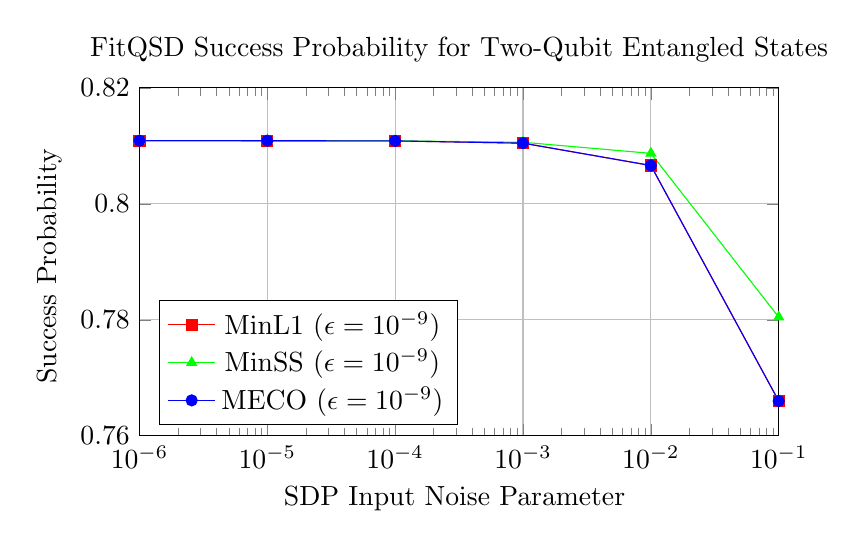
\begin{tikzpicture}
        \begin{axis}[
                xlabel={SDP Input Noise Parameter $\lSDP$},
                ylabel={Success Probability $\psucc$},
                xmode=log,
                xmin=1e-6, xmax=1e-1,
                ymin=0.76, ymax=0.82,
                grid=major,
                width=0.8\textwidth,
                height=6cm,
                legend pos=south west,
                title={FitQSD Success Probability for Two-Qubit Entangled States}
            ]
            \addplot[mark=square*, red] coordinates {
                    (1.00e-06, 0.8108929) (1.00e-05, 0.8108909) (1.00e-04, 0.8108562)
                    (1.00e-03, 0.8104668) (1.00e-02, 0.8066100) (1.00e-01, 0.7659851)
                };
            \addlegendentry{MinL1 ($\epsilon = 10^{-9}$)}
            \addplot[mark=triangle*, green] coordinates {
                    (1.00e-06, 0.8108753) (1.00e-05, 0.8108731) (1.00e-04, 0.8108618)
                    (1.00e-03, 0.8106197) (1.00e-02, 0.8087073) (1.00e-01, 0.7804561)
                };
            \addlegendentry{MinSS ($\epsilon = 10^{-9}$)}
            \addplot[mark=*, blue] coordinates {
                    (1.00e-06, 0.8108927) (1.00e-05, 0.8108889) (1.00e-04, 0.8108504)
                    (1.00e-03, 0.8104660) (1.00e-02, 0.8066098) (1.00e-01, 0.7659851)
                };
            \addlegendentry{MECO ($\epsilon = 10^{-9}$)}
        \end{axis}
    \end{tikzpicture}
    \caption{Success probability $\psucc$ versus SDP input noise $\lSDP$ for FitQSD methods on two-qubit entangled states with parameters $a_1 = 0.2$, $a_2 = 0.5$, $a_3 = 0.7$ (Subsection \ref{subsec:entangled_states}), priors $1/3$, using MOSEK at $\epsilon = 10^{-9}$. MinSS yields higher $\psucc$ but higher $L_2$ norm at low $\lSDP$ due to precision limitations.}
    \label{fig:fitqsd_results}
\end{figure}